\PassOptionsToPackage{subsection=false}{beamerouterthememiniframes}
\PassOptionsToPackage{dvipsnames,table}{xcolor}
\documentclass[fleqn]{beamer}
\usepackage{graphicx}
\usepackage{multirow}
\usepackage{multicol}
\usepackage{amsmath,amsfonts,amsthm,amsopn}
\usepackage{color, colortbl}
\usepackage{subfig}
\usepackage{wrapfig}
\usepackage{fancybox}
\usepackage{tikz}
\usepackage{fancyhdr}
\usepackage{setspace}
\usepackage{xcolor}
\usepackage{movie15}
\usepackage{pifont}
\usepackage{soul}
\usepackage{fancyvrb,newverbs}
\usepackage{epsfig}
\usepackage{epstopdf}
\fvset{fontsize=\footnotesize}
\RecustomVerbatimEnvironment{verbatim}{Verbatim}{}

%\usepackage{fancybox}

\usetheme{Szeged}
\usecolortheme{default}

%\definecolor{links}{HTML}{2A1B81}
%\definecolor{links}{blue!20}
\hypersetup{colorlinks,linkcolor=,urlcolor=blue!80}

\setbeamertemplate{blocks}[rounded]
\setbeamercolor{block title}{bg=blue!40,fg=black}
\setbeamercolor{block body}{bg=blue!10}


\newenvironment<>{clicker}[1]{%
  \begin{actionenv}#2%
      \def\insertblocktitle{#1}%
      \par%
      \mode<presentation>{%
        \setbeamercolor{block title}{fg=white,bg=magenta}
       \setbeamercolor{block body}{fg=black,bg=magenta!10}
       \setbeamercolor{itemize item}{fg=magenta}
       \setbeamertemplate{itemize item}[triangle]
       \setbeamercolor{enumerate item}{fg=magenta}
     }%
      \usebeamertemplate{block begin}}
    {\par\usebeamertemplate{block end}\end{actionenv}}

%\newcommand{\bmp}{\begin{minipage}}
%\newcommand{\emp}{\end{minipage}}
%\newcommand{\blankcolumn}{\bmp{.05\textwidth}\hspace{0.50in} \emp}

\defbeamertemplate*{footline}{infolines theme}
{
  \leavevmode%
  \hbox{%
  \begin{beamercolorbox}[wd=.333333\paperwidth,ht=2.25ex,dp=1ex,left]{author in head/foot}%
    \usebeamerfont{author in head/foot}~~\insertshortinstitute: \insertshorttitle
  \end{beamercolorbox}%
  \begin{beamercolorbox}[wd=.67\paperwidth,ht=2.25ex,dp=1ex,right]{date in head/foot}%
    \usebeamerfont{date in head/foot}%\insertshortdate{}\hspace*{2em}
    \insertframenumber{} / \inserttotalframenumber\hspace*{2ex}
  \end{beamercolorbox}
  }%
  \vskip0pt%
}

\newcommand{\cmark}{\ding{51}}%
\newcommand{\xmark}{\ding{55}}%
\newcommand{\grp}{\textcolor{magenta}{Group Exercise}}
\newcommand{\grpc}{\textcolor{magenta}{Group Exercise, continued}}
\newcommand{\bsans}[1]{\underline{\hspace{0.2in}\color{blue!80}{#1}\hspace{0.2in}}}

\definecolor{cverbbg}{gray}{0.93}
\newenvironment{cverbatim}
 {\SaveVerbatim{cverb}}
 {\endSaveVerbatim
  \flushleft\fboxrule=0pt\fboxsep=.5em
  \colorbox{cverbbg}{\BUseVerbatim{cverb}}%
  \endflushleft
}
\newenvironment{lcverbatim}
 {\SaveVerbatim{cverb}}
 {\endSaveVerbatim
  \flushleft\fboxrule=0pt\fboxsep=.5em
  \colorbox{cverbbg}{%
    \makebox[\dimexpr\linewidth-2\fboxsep][l]{\BUseVerbatim{cverb}}%
  }
  \endflushleft
}

\newcommand{\bmp}{\begin{minipage}}
\newcommand{\emp}{\end{minipage}}
\newcommand{\blankcolumn}{\bmp{.05\textwidth}\hspace{0.50in} \emp}

 \newenvironment{code}[1]%
  {\vspace{.1in}\footnotesize\Verbatim[frame=single,label=SAS Code,commandchars=\\\{\},xrightmargin=#1\textwidth,framesep=.2in,labelposition=all]}
  {\endVerbatim\normalsize}

 \newenvironment{Rcode}[1]%
  {\vspace{.1in}\footnotesize\Verbatim[frame=single,label=R Code,commandchars=\\\{\},xrightmargin=#1\textwidth,framesep=.2in,labelposition=all]}
  {\endVerbatim\normalsize}

   \newenvironment{RcodeScript}[1]%
  {\vspace{.1in}\scriptsize\Verbatim[frame=single,label=R Code,commandchars=\\\{\},xrightmargin=#1\textwidth,framesep=.2in,labelposition=all]}
  {\endVerbatim\normalsize}

 \newenvironment{RcodeTiny}[1]%
  {\vspace{.1in}\tiny\Verbatim[frame=single,label=R Code,commandchars=\\\{\},xrightmargin=#1\textwidth,framesep=.2in,labelposition=all]}
  {\endVerbatim\normalsize}


   \newenvironment{Rout}[1]%
  {\vspace{.1in}\footnotesize\Verbatim[frame=single,label=R Output,commandchars=\\\{\},xrightmargin=#1\textwidth,framesep=.2in,labelposition=all]}
  {\endVerbatim\normalsize}
  
     \newenvironment{MTout}[1]%
  {\vspace{.1in}\footnotesize\Verbatim[frame=single,label=Minitab Output,commandchars=\\\{\},xrightmargin=#1\textwidth,framesep=.2in,labelposition=all]}
  {\endVerbatim\normalsize}

   \newenvironment{RoutScript}[1]%
  {\vspace{.1in}\scriptsize\Verbatim[frame=single,label=R Output,commandchars=\\\{\},xrightmargin=#1\textwidth,framesep=.2in,labelposition=all]}
  {\endVerbatim\normalsize}

 \newenvironment{RoutTiny}[1]%
  {\vspace{.1in}\tiny\Verbatim[frame=single,label=R Output,commandchars=\\\{\},xrightmargin=#1\textwidth,framesep=.2in,labelposition=all]}
  {\endVerbatim\normalsize}

\newenvironment{craw}[2]%
{\vspace{.1in}\footnotesize\Verbatim[frame=single,label=#2,commandchars=\\\{\},xrightmargin=#1\textwidth,framesep=.2in,labelposition=all]}
  {\endVerbatim\normalsize}


\newenvironment{scriptcraw}[2]%
{\vspace{.1in}\scriptsize \Verbatim[frame=single,label=#2,commandchars=\\\{\},xrightmargin=#1\textwidth,framesep=.2in,labelposition=all]}
  {\endVerbatim\normalsize}

  \newenvironment{tinycraw}[2]%
{\vspace{.1in}\tiny \Verbatim[frame=single,label=#2,commandchars=\\\{\},xrightmargin=#1\textwidth,framesep=.2in,labelposition=all]}
  {\endVerbatim\normalsize}




\title[Set 4]{Nonparametric methods: \\ empirical survival function \\and the Kaplan-Meier estimator}
\author[Pileggi]{Shannon Pileggi}

\institute[STAT 417]{STAT 417}

\date{}


\begin{document}

\begin{frame}
\titlepage
\end{frame}

\begin{frame}
\frametitle{OUTLINE\qquad\qquad\qquad} \tableofcontents[hideallsubsections]
\end{frame}


%===========================================================================================================================
\section[Survival estimators]{Survival estimators}
%===========================================================================================================================
\subsection{}

\begin{frame}
\frametitle{Nonparametric methods}
\begin{itemize}
\item We have covered several parametric models to describe time-to-event data; however, it might not be a simple matter to assign a specific probability distribution (e.g. consider the age at first drink of alcohol).

\item In practice, when the probability distribution is not known, we will need to use \textit{nonparametric estimators} of the survival function, hazard function, and cumulative hazard functions that do not assume any form of the probability model for $T$.

\item In addition, descriptive quantities such as the mean and median will need to be estimated.

\item The main issue faced with time-to-event data is that some times may be \textit{incomplete} (censored or truncated).  We'll discuss methods and techniques that accommodate \textit{right censored} observations.

\item Why do we need to accommodate censoring?

%\item Since, right censored observations are the most common type of incomplete event times, we will discuss methods and techniques that accommodate them.

%\item First, let's see what happens when we ignore the (right) censoring.
\end{itemize}
\end{frame}

\begin{frame}
\frametitle{Example: descriptive statistics with censored values}
Consider the following extreme example: A statistics exam was administered to 10 students. At the end of the 50 minute class period, one student had finished (in 45 minutes), and the others had not finished it.
\begin{enumerate}
\item Describe the time-to-event variable $T$.
\item[] % T = time since class starts until finish exam time (minutes)
\item[]
\item What are the observed values of $T$?
\item[] % 45, 50+,  50+, etc.
\item[]
\item What distribution do you think $T$ follows?
\item[]
\item[]
\end{enumerate}
\end{frame}

\begin{frame}
\frametitle{Example: descriptive statistics with censored values, cont.}
\begin{enumerate}
\setcounter{enumi}{3}
\item Treat the right censored times as complete. Estimate the average time to complete the exam.
\item[] % mean = 49.5
\item[]
\item Throw out the right censored times. Estimate the average time to complete the exam.
\item[] % mean = 45
\item[]
\item What issues do you see with either of the strategies for dealing with censored data?
\item[] % Method 3 - doesn't account for additional length of time, sample mean is an underestimate of population mean
\item[] % Method 4 - reduces sample size, discards information from students unable to complete the exam; sample mean underestimates population mean
\item[]
\item[]
\end{enumerate}
\end{frame}

\begin{frame}
\frametitle{Estimating survival probabilities}
The following times compose a \emph{subsample} of 7 of the 57 motorist reaction times in seconds:
\begin{center}
\begin{tabular}{ccccccc}
%Motorist & 1 & 2 & 3 & 4 & 5 & 6 & 7\\ \hline
$1.41$ & $1.41+$ & $2.76+$ & $3.56$ & $4.18$ &  $4.71+$   & $13.18$ \\
\end{tabular}
\end{center}
Estimate the probability that a motorist takes longer than 1.41 seconds to react aggressively under each of the following schemes:
\begin{enumerate}
\item Treat the censored times as complete.
\item[] % Pr(T>1.141) = 5/7
\item[]
\item Throw out the censored times.
\item[] % Pr(T>1.141) = 3/4
\item[]
%We'll compare these values to proper estimate later
\end{enumerate}
\end{frame}



\begin{frame}
\frametitle{Estimators of the survival function}
\begin{itemize}
%\item We'll come back to estimates of mean survival time later.
\item Recall that the primary function used to describe the time-to-event variable $T$ is the survival function, $S(t)=P(T>t)$.

\item When we treat all times as complete (\# 1 in previous example), this  illustrates one strategy or method for estimating $S(t)$ known as the \textbf{empirical survival function (ESF)}, denoted $\widehat{S}_E(t)$.
\item $\widehat{S}_E(t)$ is typically calculated for each observed time $t_i$ in the sample, and then plotted as a \textit{step function}.
\item Note: this method is unbiased for $S(t)$ \textbf{if}...
\end{itemize}
%\textbf{Empirical Survival Function}: Let $t_1,t_2,\ldots,t_n$ represent the observed event times for $n$ individuals (includes censored and complete times). The ESF, $\widehat{S}_E(t)$, is calculated as:
\vskip100pt
\end{frame}

\begin{frame}
\frametitle{Empirical survival function}
 Let $t_1,t_2,\ldots,t_n$ represent the observed event times for $n$ individuals (includes censored and complete times). The ESF, $\widehat{S}_E(t)$, is calculated as:
\vskip200pt
\end{frame}


\begin{frame}
\frametitle{Empirical survival function, motorist reaction times example}
\begin{center}
\begin{tabular}{ccccccc}
%Motorist & 1 & 2 & 3 & 4 & 5 & 6 & 7\\ \hline
$1.41$ & $1.41+$ & $2.76+$ & $3.56$ & $4.18$ &  $4.71+$   & $13.18$ \\
\end{tabular}
\end{center}
\begin{enumerate}
\item Find $\widehat{S}_E(t)$ for each value of $t_i$.
%\item Sketch the graph of $\widehat{S}_E(t)$ for all $t$.
%\item Using the graph, estimate $S(2)$, $S(6)$, and $S(10)$.
\end{enumerate}
\vskip200pt
\end{frame}

\begin{frame}
\frametitle{Empirical survival function, motorist reaction times example, cont.}
\begin{enumerate}
\setcounter{enumi}{1}
%\item Find $\widehat{S}_E(t)$ for each value of $t_i$.
\item Sketch the graph of $\widehat{S}_E(t)$ for all $t$.
\item Using the graph, estimate $S(2)$, $S(6)$, and $S(10)$.
\end{enumerate}
\vskip200pt
\end{frame}

\begin{frame}
\frametitle{Summary: ignoring censored event times}
\begin{itemize}
\item By treating the censored times as complete times, we are assuming that the event times are shorter than what they actually are, thereby underestimating the true quantities, e.g. mean survival time and
probabilities of survival.
\item By disregarding the censored times, we lose information about the event times (consider the statistics exam times).
\item Treating the censored observations as complete or ignoring them will \textit{bias} any estimates based on the remaining complete times.
\item[]
\end{itemize}
Next we'll consider a way to estimate the survival probabilities with a method that take into account the censoring status of
subjects.
\end{frame}

%===========================================================================================================================
\section[KM estimator]{Kaplan-Meier estimator}
%===========================================================================================================================
\subsection{}
\begin{frame}
\tableofcontents[currentsection, hideallsubsections]
\end{frame}

\begin{frame}
\frametitle{Kaplan-Meier estimator}
\begin{itemize}
\item The \textbf{Kaplan-Meier estimator}, denoted $\widehat{S}(t)$, adjusts $\widehat{S}_E(t)$ to reflect the presence of right censored observations.
\item When constructing $\widehat{S}(t)$, denote the $n$ observed event times as $t_1, t_2, \ldots, t_n$, and the number of distinct \textit{complete} event is $m$, where $m \leq n$.
\end{itemize}
\begin{center}
\begin{tabular}{ccccccc}
%Motorist & 1 & 2 & 3 & 4 & 5 & 6 & 7\\ \hline
$1.41$ & $1.41+$ & $2.76+$ & $3.56$ & $4.18$ &  $4.71+$   & $13.18$ \\
\end{tabular}
\end{center}
\begin{clicker}{In the motorist reaction time subsample, $m=$\underline{\hspace{0.5in}} and $n=$\underline{\hspace{0.5in}}.}
\begin{enumerate}
\item $m=6$, $n=7$
\item $m=7$, $n=6$
\item $m=4$, $n=7$ %correct
\item $m=5$, $n=7$
\end{enumerate}
\end{clicker}
\end{frame}


\begin{frame}
\frametitle{Kaplan-Meier estimator, cont.}
\begin{itemize}
\item Then the \textit{ordered} complete event times from smallest to largest are denoted as:
\item[]
\item[]
\item[] with the convention that $t_{(0)}=0$.
\item Using the complete times, $t_{(1)}$ through $t_{(m)}$, and beginning with time $t_{(0)}=0$, create a series of time intervals:
\item[]
\item[]   %$[0,t_{(1)}), [t_{(1)}, t_{(2)}),\ldots$,
\item[]   with some modifications to the last interval depending on whether the largest observed time is complete or censored.
%are used to define
%intervals beginning at one complete event time, and ending just
%prior to the next complete event time with some minor modifications
%for the first and last intervals.
\end{itemize}
\end{frame}


\begin{frame}
\frametitle{Kaplan-Meier estimator, cont.}
\begin{itemize}
\item By convention, the $0^{th}$ time interval is $[0,t_{(1)})$
\item If the largest observed time is complete (denoted $t_{(m)}$), then the last ($m^{th}$) interval is $[t_{(m)},t_{(m)}]$.
\item If the largest observed time is censored (denoted $t_{\mbox{max}}+$), then the last interval is $[t_{(m)},t_{\mbox{max}}+)$.
\end{itemize}
\end{frame}


\begin{frame}
\frametitle{Kaplan-Meier estimator example}
\begin{center}
\begin{tabular}{ccccccc}
%Motorist & 1 & 2 & 3 & 4 & 5 & 6 & 7\\ \hline
$1.41$ & $1.41+$ & $2.76+$ & $3.56$ & $4.18$ &  $4.71+$   & $13.18$ \\
\end{tabular}
\end{center}
\begin{enumerate}
\item  List the values corresponding to $t_{(1)}$ through $t_{(m)}$.
\item[]
\item[]
\item[]
\item Write out the time intervals.
\end{enumerate}
\vskip200pt
\end{frame}

\begin{frame}
\frametitle{Kaplan-Meier estimator, cont.}
%Only those individuals who experience the target event contribute to the estimator.
Once the complete event times have been identified, and the $m$ time intervals have been constructed, then for
$i=0,\dots,m$, define:
\begin{itemize}

\item $n_i$
\item[]
\item[]
%the number of individuals at risk (who haven't experienced the event) just prior to time $t_{(i)}$, i.e.
%just prior to the $i^{th}$ time interval.

\item $d_i$
\item[]
\item[]
%the number of individuals who \textit{have} experienced the event (fail) at time $t_{(i)}$.

\item $n_i-d_i$
\item[]
\item[]
%the number of individuals who \textit{haven't} experienced the event (survive) just prior to time
%$t_{(i)}$.

%\item Then create a table containing the quantities: $t_{(i)}$, $n_i$, $d_i$, and $n_i-d_i$


%The proportion who survive at time t_(i)

%\item  By convention, the {first interval} begins at time $t_0=0$, and
%ends just prior to the time when the first event occurs, time $t_1$.
%This interval is denoted by $[0, t_1)$.
%\item If the largest event time is censored, then the
%interval extends to this censored time, but the interval is open on
%the right, i.e. the interval is given by $[t_m, \mbox{``largest censored time in the data set"})$. If the largest observed event time is complete, then the {last interval} is technically not an interval, and just consists of a single point, i.e. the interval is given by $[t_m, t_m]$.
%\item The {intervals between the first and last} are created using the remaining
%complete event times as endpoints, i.e. $[t_{i-1}, t_{i})$, for $i =
%2, 3,\ldots, m-1$. If there are ties in the data, (i.e. two
%complete times are identical), then one interval will contain
%more than one complete event time.
\end{itemize}
%\textbf{Example: Motorist Reaction Times (Subsample)}. For the sample of motorist reaction times,  in the table on the next slide. Leave the columns for $\hat{p}_i$ and $\widehat{S}(t)$ empty for now.
%\vskip .9in
%estimated probability of surviving through the $i^{th}$ interval, conditional on surviving to the beginning of the $i^{th}$ interval.
\end{frame}

\begin{frame}
\frametitle{Kaplan-Meier estimator example, cont.}
\hspace*{-0.3in}
{\renewcommand{\arraystretch}{2.0}
\begin{tabular}{|c|c|c|c|c|c|c|c|}
\hline
$i$ & Interval & $t_{(i)}$ & $~~n_i~~$ & $~~d_i~~$ & $n_i-d_i$ &$~~\hat{p}_i~~$ & $~~\widehat{S}(t_{(i)})~~$ \\
\hline
0 & $[0,1.41)$ & 0 &  &  & & &\\
\hline
1 & $[1.41,3.56)$ & 1.41 & &  &  & &  \\
\hline
2& $[3.56,4.18)$ & 3.56 & & &  &  & \\
\hline
3 & $[4.18,13.18)$ & 4.18 & & & & &\\
\hline
4 & $[13.18,13.18]$ & 13.18 & & & & &\\
 \hline
\end{tabular}}
\end{frame}



\begin{frame}
\frametitle{Kaplan-Meier estimator, cont.}
How would we evaluate $S(t)$ at the complete event times: $t_{(1)}, \ldots, t_{(m)}$?
\begin{itemize}
\item[]
\item Recall the definition of the survival function:
\item[]
\begin{eqnarray}
{S(t)=P(T>t)} \nonumber
\end{eqnarray}
\item[]
\item Then $S(t_{(1)}), S(t_{(2)}), \ldots, S(t_{(m)})$ can each be written as a product of conditional probabilities
 using applications of the \textbf{multiplication rule}:
 \item[]
 \item[]
 \item[]
%P(A & B) = P(A)P(B|A)

\item Note: by definition: $S(t_{(0)})=P(T>0)=1$.
\end{itemize}
\end{frame}


\begin{frame}
\frametitle{Kaplan-Meier estimator, cont.}
Then using the multiplication rule we can write
$S(t_{(1)})=P(T>t_{(1)})$ as:
\vskip200pt
\end{frame}


\begin{frame}
\frametitle{Kaplan-Meier estimator, cont.}
Furthermore:
\begin{itemize}
\item $S(t_{(2)})=P(T>t_{(2)})=$
\item[]
\item[]
\item[]
\item Finally we have $S(t_{(i)})=P(T>t_{(i)})=$
\item[]
\item[]
\item[]
\end{itemize}
We'll need estimates of:
\begin{eqnarray}
P(T>t_{(i)}|T>t_{(i-1)}) \nonumber
\end{eqnarray}
for $i=1,\ldots,m$.
\end{frame}


\begin{frame}
\frametitle{$\widehat{S}(t)$: motorist reaction times}
Using the information in the table, estimate the probability that a motorist will not react aggressively after 1.41 seconds, given that the motorist hasn't reacted aggressively after 0 seconds.
%estimate P(T>t_(1)|T>t_(0)) = #haven't reacted agg after 1.41 seconds/#haven't reacted agg after 0 seconds = (n_1-d_1)/n_1 = (7-1)/7
\vskip200pt
\end{frame}


\begin{frame}
\frametitle{Kaplan-Meier estimator, cont.}
\begin{itemize}
\item[] The estimate of $P(T>t_{(i)}|T>t_{(i-1)})$, denoted by $\hat{p}_i$ is given by:
\item[]
\item[]
%\begin{eqnarray}
%\hat{p}_j = (n_j-d_j)/n_j \nonumber
%\end{eqnarray}
\item[] This is the estimated conditional probability of an individual surviving past time $t_{(i)}$ given that the individual has survived past
time $t_{(i-1)}$.
\item[]
\end{itemize}
\textbf{Example:}  Calculate the values of $\hat{p}_i$ and fill in the table.
\vskip 1.6in
\end{frame}

\begin{frame}
\frametitle{Kaplan-Meier estimator, cont.}
Hence, the Kaplan-Meier estimator of the survival function at the complete event time $t_{(i)}$ is given by:
\vskip50pt
%\begin{eqnarray}
%{\widehat{S}(t_{(i)})=\prod_{j=1}^i \hat{p}_j}  \nonumber
%\end{eqnarray}
or for general time $t$, the Kaplan-Meier estimator is given by:
\vskip50pt
%\begin{eqnarray}
%\boxed{\widehat{S}(t)=\prod_{t_{(i)} \leq t} \hat{p}_i}  \nonumber
%\end{eqnarray}

\end{frame}

\begin{frame}
\frametitle{Kaplan-Meier example, cont.}
Compute the values of $\widehat{S}(t_{(i)})$ and fill in the last column in the table.
\vskip200pt
\end{frame}

\begin{frame}
\frametitle{Kaplan-Meier notes}
\begin{enumerate}
\item $\widehat{S}(t)=1$ for $t < t_{(1)}$.
\item[]
\item $\widehat{S}(t)$ remains constant for $t_{(i)} \leq t < t_{(i+1)}$.
%i.e. $\widehat{S}(t)$ remains constant within the $i^{th}$ interval.
\item[]
\item The Kaplan-Meier estimates of survival probability are always greater than or equal to estimates based on the empirical survival function.
\item[]
\item If no censoring is present in the data, then the Kaplan-Meier and empirical survival functions are identical. What do you think happens when all the times are (right) censored?
\end{enumerate}
\end{frame}

\begin{frame}
\frametitle{\grp}
\begin{clicker}{Will $\widehat{S}(t)$ reach 0?}
\begin{enumerate}
\item yes
\item no
\item it depends %correct
%If largest event time is complete, then S(t) will reach 0.
%If largest event time is censored, then S(t) will not reach 0.
\end{enumerate}
\end{clicker}
\vskip100pt
\end{frame}

\begin{frame}
\frametitle{Comparing ESF and KM estimators}
Use both the ESF and KM estimators to estimate $S(2)$, $S(6)$, and $S(10)$.  How do the estimates compare?
\vskip10pt
{\renewcommand{\arraystretch}{2.0}
\begin{tabular}{|c|c|c|}
\hline
 & ~~$\widehat{S}_E(t)$ (ESF)~~ & ~~$\widehat{S}(t)$ (KM)~~ \\
 \hline
$\hat{S}(2)$ & & \\
\hline
$\hat{S}(6)$ & & \\
\hline
$\hat{S}(10)$& & \\
\hline
\end{tabular}}
\end{frame}


%===========================================================================================================================
\section[KM in Minitab/R]{KM in Minitab/R}
%===========================================================================================================================
\subsection{}
\begin{frame}
\tableofcontents[currentsection, hideallsubsections]
\end{frame}

\begin{frame}
\frametitle{Graphs of the survival estimators}
The \textbf{Kaplan-Meier curve} is a graphical display of $\widehat{S}(t)$, and is a (right continuous) step function which steps down only at \textit{complete} event times.\\
\vskip5pt
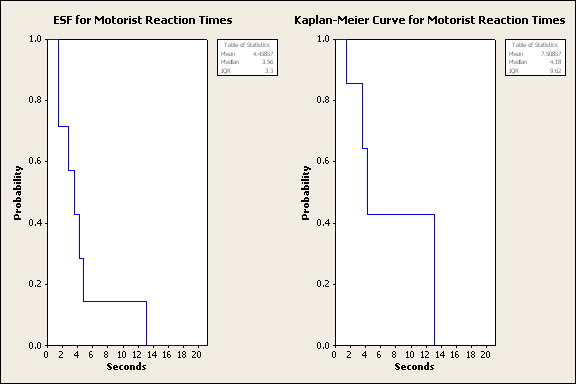
\includegraphics[width=0.70\textwidth]{Figures/esf_km_motorist.jpg}
\end{frame}


\begin{frame}[fragile]
\frametitle{Minitab: Kaplan-Meier estimates}
Minitab output for the \texttt{Nonparametric Distribution Analysis} of the subsample of motorist reaction times:
\vskip10pt
\begin{verbatim}
    Distribution Analysis: Time
    Variable: Time

    Censoring Information  Count
    Uncensored value           4
    Right censored value       3

    Censoring value: Censor 1 = 0
\end{verbatim}
\end{frame}

\begin{frame}[fragile]
\frametitle{Minitab: Kaplan-Meier estimates}
\begin{verbatim}
    Nonparametric Estimates

    Characteristics of Variable

                Standard   95.0% Normal CI
    Mean(MTTF)     Error    Lower    Upper
       7.50857   2.54935  2.51194  12.5052

    Median = 4.18
    IQR = 9.62  Q1 = 3.56  Q3 = 13.18
\end{verbatim}
\end{frame}

\begin{frame}[fragile]
\frametitle{Minitab: Kaplan-Meier estimates}
\begin{verbatim}
    Kaplan-Meier Estimates

            Number  Number     Survival  Standard   95.0% Normal CI
     Time  at Risk  Failed  Probability     Error     Lower    Upper
     1.41        7       1     0.857143  0.132260  0.597918  1.00000
     3.56        4       1     0.642857  0.210424  0.230433  1.00000
     4.18        3       1     0.428571  0.224258  0.000000  0.86811
    13.18        1       1     0.000000  0.000000  0.000000  0.00000
\end{verbatim}
\end{frame}


\begin{frame}
\frametitle{Describing survival experiences}
The following slide (from left-right, top-bottom) provides $\widehat{S}(t)$ for the four example data sets:
\begin{enumerate}
    \item Age at first drink of alcohol
    \item Seconds until driver reacts aggressively
    \item Days until death from lung cancer (North Central Cancer Treatment Group Study)
    \item Months until rearrest
\end{enumerate}
Examine the Kaplan-Meier curves for each data set.  Comment on some notable features of the ``survival" experiences of a couple of the examples (in particular the rearrest data).
\end{frame}


\begin{frame}
\frametitle{Describing survival experiences}
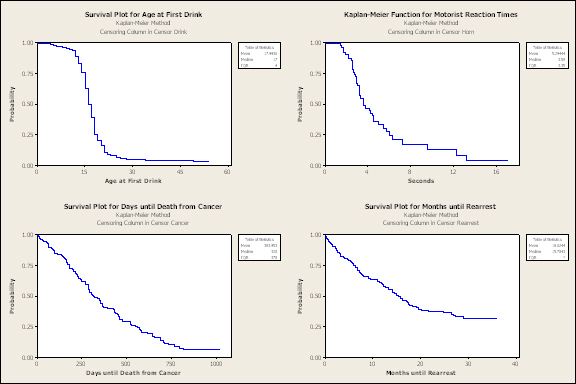
\includegraphics[width=0.85\textwidth]{Figures/KM_four_datasets.jpg}
\end{frame}


\begin{frame}
\frametitle{Describing survival experiences}
\end{frame}

\begin{frame}[fragile]
\frametitle{Kaplan-Meier estimates using \texttt{R}}
\textbf{Motorist reaction times example: R code}
\begin{verbatim}
 > library(survival)
 > time <- c(1.41,1.41,2.76,3.56,4.18,4.71,13.18)
 > censor <- c(1,0,0,1,1,0,1)
 > motorist_surv <- Surv(time,censor)
 > KM_obj <- survfit(motorist_surv~1, conf.type="none")
 > summary(KM_obj)
\end{verbatim}
\vskip5pt
\textbf{R output:}
\begin{verbatim}
    Call: survfit(formula = motorist.surv ~ 1, conf.type = "none")

      time n.risk n.event survival std.err
      1.41      7       1    0.857   0.132
      3.56      4       1    0.643   0.210
      4.18      3       1    0.429   0.224
     13.18      1       1    0.000     NaN
\end{verbatim}
\end{frame}

\begin{frame}[fragile]
\frametitle{Kaplan-Meier estimates using \texttt{R}}
\textbf{Motorist reaction times example: R code}
\begin{verbatim}
 > plot(KM_obj, xlab="Seconds", ylab="Survival Probability",
     main="KM Curve")
\end{verbatim}
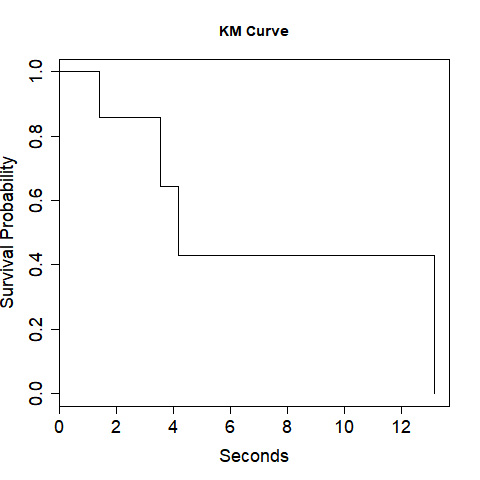
\includegraphics[width=0.50\textwidth]{Figures/KM_curve_samp_motorist.png}
\end{frame}


\end{document} 